\section{The IoT era with low-cost IoT for all}

\subsection{IoT connectivity made easy}

Recent Low-Power Wide Area Networks (LPWAN) technologies for Internet-of-Things (IoT) introduced by Sigfox and Semtech's (LoRa\texttrademark) are currently gaining incredible interest and are under intense deployment campaigns worldwide. They definitely initiated a new innovation cycle as they obviously provide a much better connectivity answer for IoT (most of IoT devices have small amount to data to send and very limited battery power) compared to traditional cellular-based connectivity (e.g. GSM/GPRS/3G) or short-range technologies such as IEEE 802.15.4. They offer several kilometers range without relay nodes to reach a central gateway, thus greatly simplifying large-scale deployment of IoT devices as opposed to the complex multi-hop approach needed by short-range radio technologies. Fig. \ref{figure-1hop} shows a typical extreme long-range 1-hop connectivity scenario to a long-range gateway, which is the single interface to Internet servers, using low-cost LoRa radio modules available from many vendors. Most of these long-range technologies can achieve 20km or higher range in line-of-sight (LOS) condition and about 2km-4km in non-LOS conditions \cite{semtech-test,Libelium-lora-web} such as in dense urban/city environments.

\begin{figure}[htb]  
\centering  
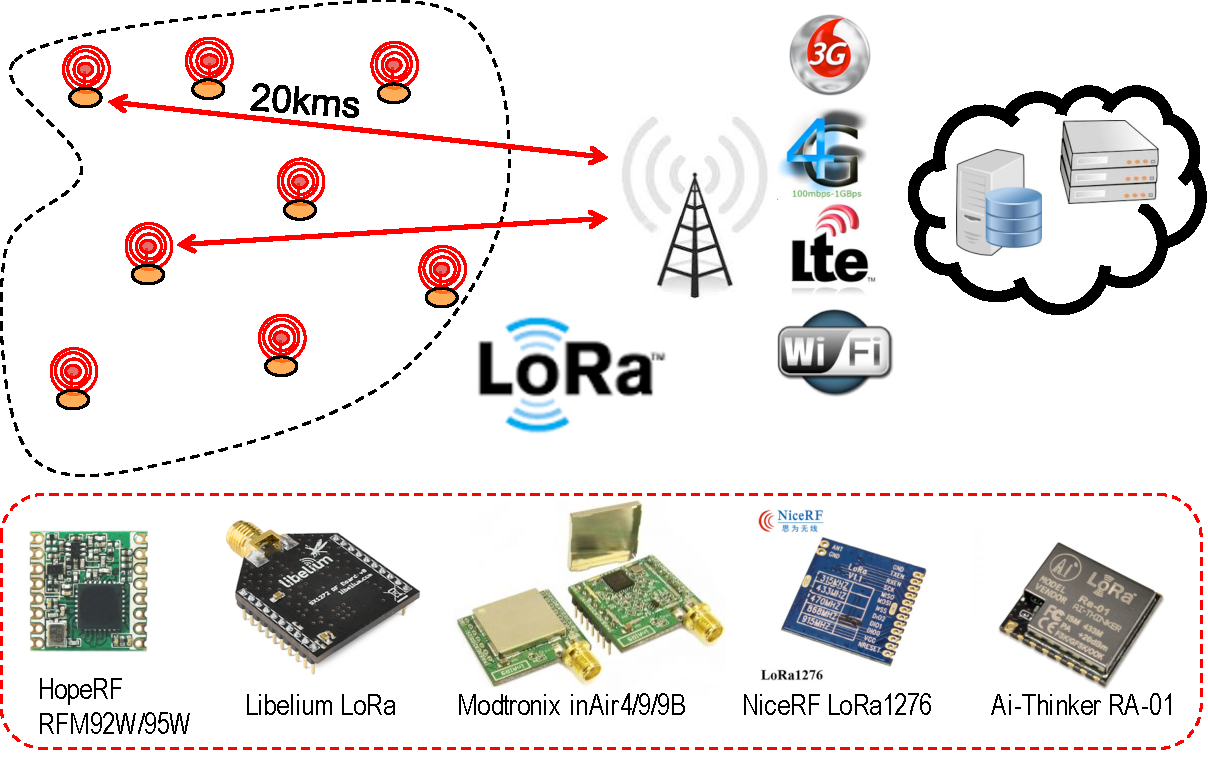
\includegraphics[width=.6\linewidth]{figures/1-hop}   
\caption{Extreme long-range application with new radio technologies}   
\label{figure-1hop}  
\end{figure} 

\subsection{Low-cost DIY IoT hardware}

Commercial IoT devices are getting mature but they are definitely too expensive for very low-income countries. In addition, these highly integrated devices are difficult to repair with their parts being hardly locally replaced.  The availability of low-cost, open-source hardware platforms such as Arduino boards definitely pushes for a Do-It-Yourself (DIY) and "off-the-shelves" design approach for a large variety of IoT applications. The Arduino ecosystem is large and proposes various board models, from large and powerful prototyping boards to smaller and less energy-consuming boards for final integration purposes as illustrated in Figure \ref{figure-generic-iot}. For instance, the small form factor Arduino Pro Mini board based on an ATmega328 microcontroller has a high performance/price tradeoff and can be used to build a low-cost generic sensing IoT platform with LoRa long-range transmission capability for about 7 euro: 2 euro for the Arduino and 5 euro for the radio module!

\begin{figure}  
\centering  
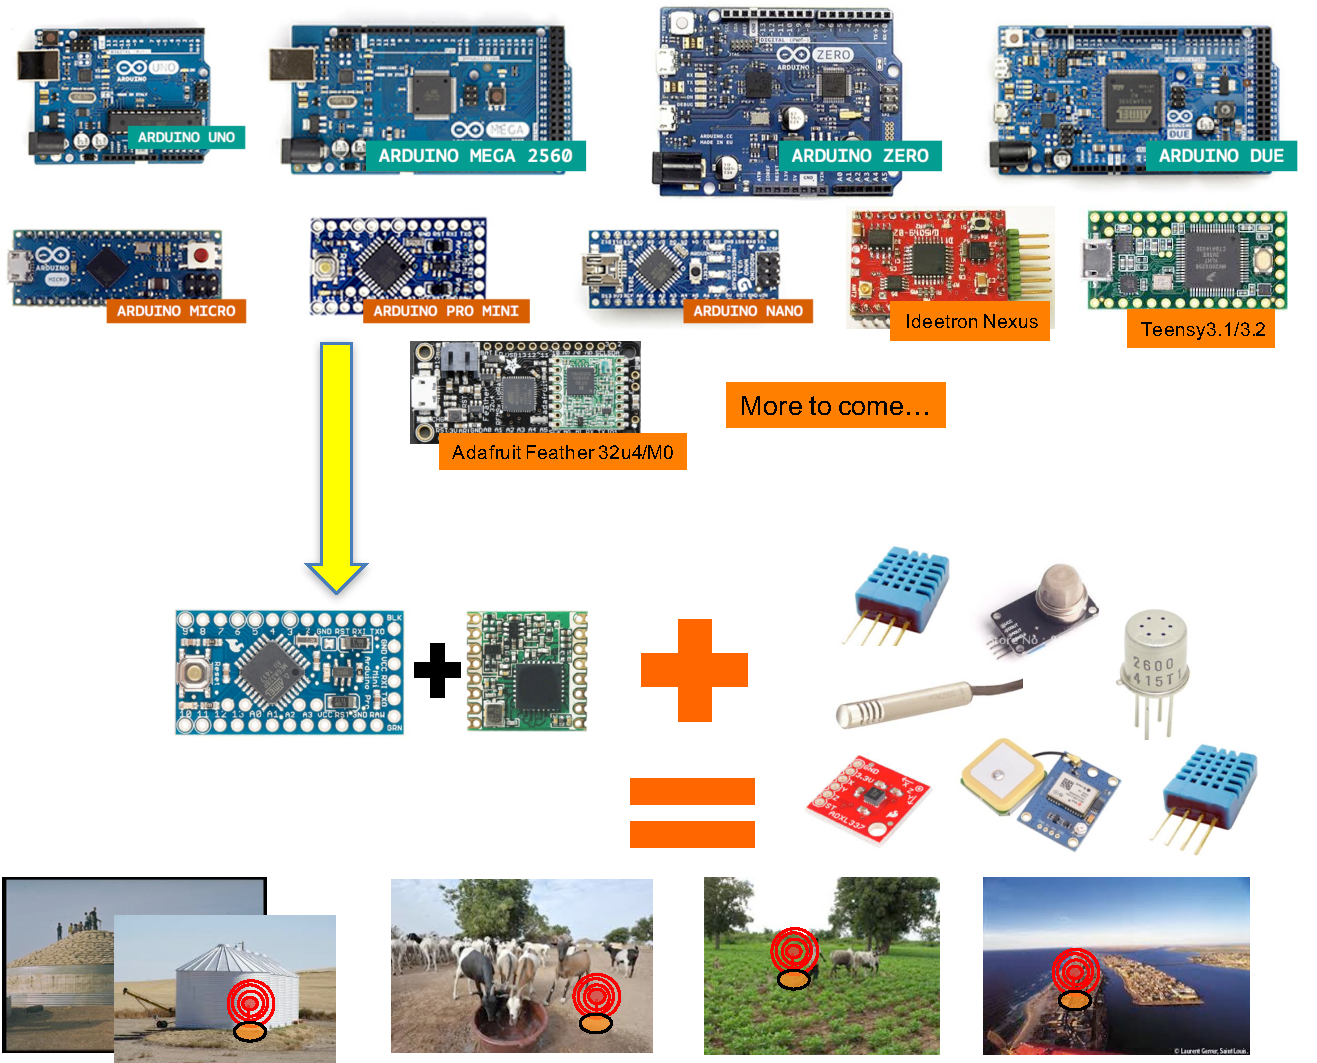
\includegraphics[width=.75\linewidth]{figures/generic-iot}   
\caption{Generic low-cost IoT hardware}   
\label{figure-generic-iot}  
\end{figure} 

Integration of these generic IoT becomes straightforward and the Arduino Pro Mini is available in the 3.3v \& 8MHz version for much lower power consumption, offering the possibility of running for more than a year on 4 AA regular batteries as illustrated in Fig. \ref{figure-easy-integration}. 

\begin{figure} 
\centering  
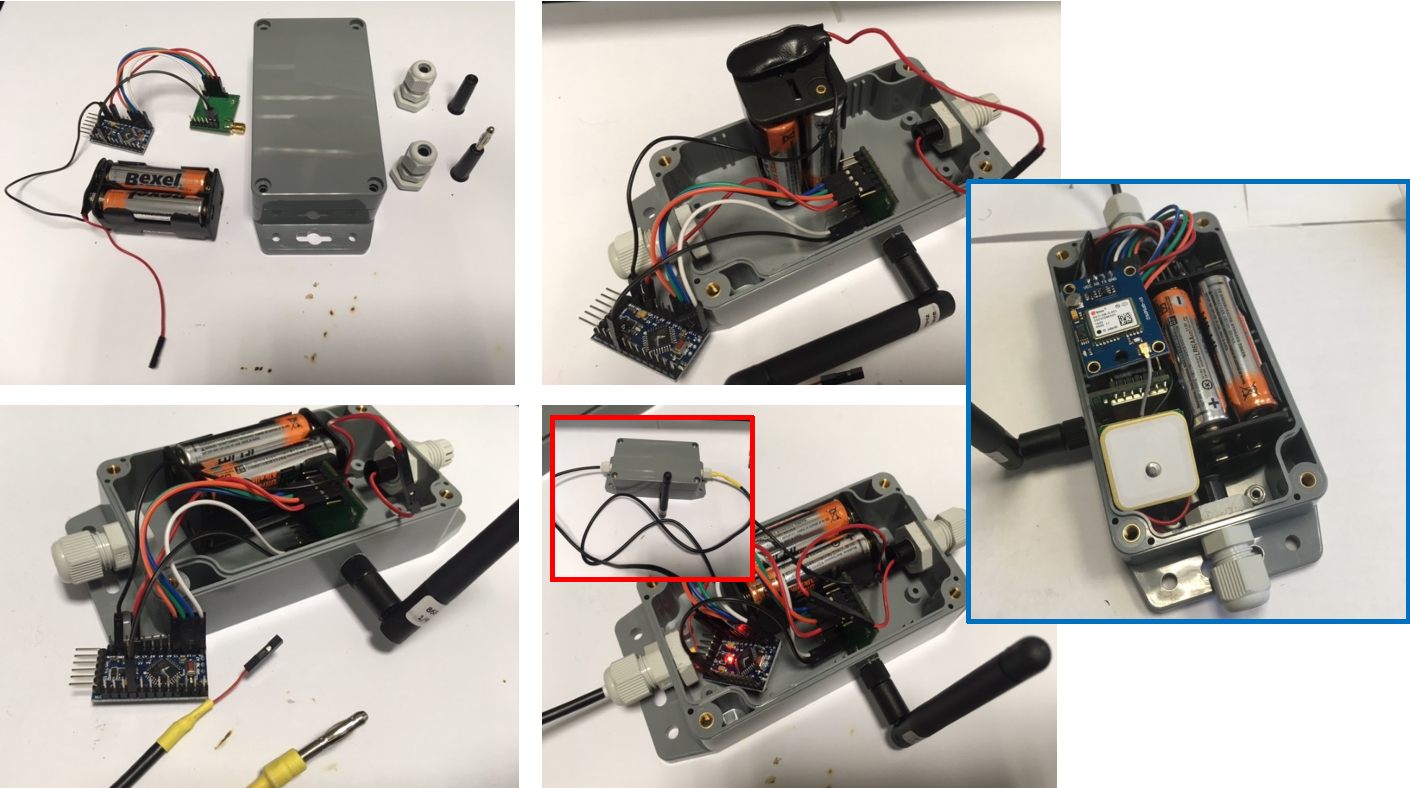
\includegraphics[width=.8\linewidth]{figures/easy-integration}   
\caption{Easy integration with DIY approach for maximum appropriation}   
\label{figure-easy-integration}  
\end{figure} 

It is expected that this availability of low-cost DIY IoT will create a tremendous uptake of the technology on a large-scale, for a large variety of applications, including those from developing countries as even a limited deployment of IoT devices can have huge impacts.

\subsection{Hardware and Software Security}
In a large scale IoT platform, that consists of local and global clouds, providing security is a challenge. A local cloud is connected to one or several IoT gateways that are close to local cloud. 

An IoT gateway is a wireless based on 4G/3G communications; thus, we cannot build a local/private network space with Local Cloud even. Somehow we need to have a public endpoint to access Orion from the Internet. Therefore, even in local cloud model we need a public endpoint. Even in local cloud model, we need a public IP or the IoT gateway would have to be in the local network.
In our platform, global cloud provides the main data broker (global Orion context broker) which receives data from distributed IoT gateways. IoT gateway communications with global Orion need to pass through the Internet. If Orion is exposed to the outside world using a public IP address of platform, then all access to Orion have to be controled in such a way to allow only authorized accesses, and deny non-authorized ones.

One way to provide security for such a communication is to use FIREWALL, and allow IP addresses of IoT gateways to be able to access Orion endpoint (e.g. public IP of platform: Orion Port). And then, deny all other accesses to Orion. Since we know that which IoT gateways are connected, or would like to connect to our platform this is a solution. At the end, we are enforcing access control to Orion by design with this solution. However, one issue can come from gateway with Internet access through a 3G dongle where the IP address is not always the same, and it may change. 

Generally, we can distinguish two scenarios for local cloud:
\begin{itemize}

\item 1) Connected with limited bandwidth (typically charged by transmitted data): Here we use local cloud to optimize for data usage because connecting to internet is expensive and slow. Data are transferred to local cloud from internet, but that's low amount compared to what would be needed to access the dashboard remotely. Here the local cloud need a public IP or we will have to implement a method to circumvent NATs. This would mean the local cloud periodically pull the data from global cloud with static public IP or it keeps an open connection to a cloud with static public IP. Data go from the IoT gateway to the global cloud and from there to the local cloud.

\item 2) Disconnected IoT gateway: In this case, the gateway must be connected with some local communication means (e.g. wifi, ethernet or LoRA) to the local network of the local cloud.
\end{itemize}

Therefore, it is important to have a co-design from hardware and software experts in place in order to address different scenarios.

Relying on IP address is not really good in some cases. There is another way in which we can rely in defining gateway id, and accepting only upload from registered gateways. It is easy to add a field in the message, to have the gateway id; thus, we can define access policies based on registered Gateway ids. For that, at platform, we need to receive the message, decode it and see if it is from a registered gateway id to let the communication happen. For this case, Gateway ID plus secure token sounds good for simple security. Alternatively, we could go for certificates. This would go nicely with securing the communication to go over SSL. To be sufficiently secure, we should communicate over HTTPS and use certificates. Since an IoT gateway is a Linux machine, we can certainly do the certificates and HTTPS.

This would mean that we have our own Certification Authority (CA). From this, we would generate certificates for the Orion and the gateway. Then we would setup both the parties to require that the opposite party presents a certificate signed by the CA.

This would have two benefits: 1) proper authentication, and 2) securing data during transport.